\documentclass{beamer}
% \documentclass[class=beamer, crop=false, notes]{standalone}

\usetheme{JuanLesPins}

% --- Languages & Fonts ---
\usepackage{polyglossia}

\newfontfamily\greekfont[Script=Greek]{Linux Libertine O}
\newfontfamily\greekfontsf[Script=Greek]{Linux Libertine O}
\newfontfamily\greekfonttt[Script=Greek]{Linux Libertine Mono O}

\setdefaultlanguage{greek}
\setotherlanguage{english}

\usepackage{caption}
\captionsetup[figure]{font=scriptsize}

% --- Cover ---
\title{Concordia}
\subtitle{Αυτόνομο κοινωνικό δίκτυο\\βασισμένο σε τεχνολογίες αποκέντρωσης}

\definecolor{concordia}{RGB}{11, 37, 64}

\newcommand{\keyword}[1]{\textbf{\textcolor{concordia}{#1}}}

\author{Νικολαΐδης Παναγιώτης \and Φανάκης Απόστολος}

\institute{
	Αριστοτέλειο Πανεπιστήμιο Θεσσαλονίκης\newline
	Τμήμα Ηλεκτρολόγων Μηχανικών και Μηχανικών Υπολογιστών
}

\date{Θεσσαλονίκη \the\year}

\begin{document}

\frame{\titlepage}

\begin{frame}
	\frametitle{Table of Contents}
	\tableofcontents
\end{frame}

\note{
	Αρχικά θα παρουσιάσουμε τα προβλήματα της σύγχρονης διαδικτυακής επικοινωνίας και θα ορίσουμε τους στόχους της εργασίας. Έπειτα, θα παρουσιάσουμε την προτεινόμενη λύση, την υλοποίηση αυτής και τη διαδικασία ανάπτυξης. Τέλος, θα μιλήσουμε για τις γνώσεις που αποκτήσαμε από τη δουλειά αυτή και θα αναφέρουμε ανοιχτά θέματα.
}

\section{Ορισμός του προβλήματος}
\begin{frame}
	\frametitle{Ορισμός του προβλήματος}
	\vspace{-\baselineskip}

	Προβλήματα στις σύγχρονες εφαρμογές αρχιτεκτονικής client-server:
	\begin{itemize}
		\item Αδύναμη ασφάλεια η οποία δεν αποτελεί προτεραιότητα
		\item Καμία εγγύηση διαθεσιμότητας
		\item Απαίτηση εμπιστοσύνης προς τον εξυπηρετητή
		\item Μη αυθεντικοποίηση των δεδομένων
		\item Έλλειψη ή/και καταπάτηση ελευθερίας του λόγου
	\end{itemize}
\end{frame}

\note{
	Μέσα από τις συζητήσεις μας με τον κύριο Δημάκη, αλλά και από τις εμπειρίες μας στον σύγχρονο διαδικτυακό διάλογο, έγινε σαφής η αδυναμία των κεντροποιημένων πλατφόρμων επικοινωνίας να αποδώσουν ορισμένα χαρακτηριστικά που είναι βασικά για την ελευθερία και την ισότητα στη συμμετοχή. Αναγνωρίσαμε ότι, μερίδα των προβλημάτων προκύπτει λόγω της σχέσης πελάτη-εξυπηρετητή που επικρατεί στις πλατφόρμες αλλά και των προτεραιοτήτων που θέτουν οι εταιρίες πίσω από αυτές.

	Συγκεκριμένα, η ασφάλεια είναι συχνά στόχος χαμηλής προτεραιότητας. Η διαθεσιμότητα πλήττεται σημαντικά καθώς ο εξυπηρετητής μπορεί ανά πάσα στιγμή να χάσει τα δεδομένα ή να αρνηθεί την πρόσβαση σε αυτά. Όλη η αρχή λειτουργίας των κεντροποιημένων αυτών συστημάτων απαιτεί την εμπιστοσύνη από τους πελάτες προς τους εξυπηρετητές, ενώ επίσης ελάχιστες είναι οι πλατφόρμες που επιτρέπουν την αυθεντικοποίηση των δεδομένων από τους χρήστες, (κάτι που τεχνολογικά είναι αρκετά εύκολο). (η αυθεντικοποίηση αφορά τον έλεγχο από τον παραλήπτη ότι ένα μήνυμα είναι γνήσιο και προέρχεται πράγματι από τον αποστολέα)

	Τέλος, ο εξυπηρετητής διατηρεί τον πλήρη έλεγχο της συμμετοχής στον διάλογο και μπορεί να αποκλείσει οποιονδήποτε χρήστη ή οντότητα από αυτόν.
}

\section{Στόχος της εργασίας}
\begin{frame}
	\frametitle{Στόχος της εργασίας}
	\vspace{-\baselineskip}

	Στόχος η δημιουργία μίας πρότυπης αυτόνομης, πλήρως αποκεντρωμένης κοινωνικής πλατφόρμας.
	\vspace{\baselineskip}

	Βασικά χαρακτηριστικά:
	\begin{itemize}
		\item Πρότυπη εφαρμογή (Proof of Concept)
		\item Πλήρης ελευθερία του λόγου
		\item Κυριότητα των χρηστών επί των δεδομένων τους
		\item Δυνατότητα διενέργειας αυθεντικών δημοκρατικών διαδικασιών
		\item Κρυπτογραφική εγγύηση αρτιότητας δεδομένων
		\item Αποκεντρωμένη αρχιτεκτονική
	\end{itemize}
\end{frame}

\note{
	Μέσα από την εργασία αυτή, στοχεύσαμε στην διερεύνηση του χώρου και στην πρότυπη υλοποίηση μίας λύσης που να αντιμετωπίζει/διευθετεί τα προβλήματα αυτά.

	Το επιθυμητό αποτέλεσμα ήταν η δημιουργία μίας ψηφιακής κοινότητας στην οποία ο ρόλος του εξυπηρετητή καθίσταται περιττός. Στην νέα πλατφόρμα αυτή, οδηγοί και διαχειριστές της συζήτησης είναι οι χρήστες οι οποίοι ως ηλεκτρονικοί πολίτες πρώτης κατηγορίας διατηρούν τον έλεγχο και την κυριότητα των δεδομένων που παράγουν. Βασικό χαρακτηριστικό της πλατφόρμας αποτελεί η δυνατότητα αυτοδιαχείρισης μέσα από αμεσοδημοκρατικές ψηφοφορίες.

	Έπειτα από διερεύνηση, συνειδητοποιήσαμε ότι οι στόχοι αυτοί είναι υλοποιήσιμοι και επικουρούνται μέσα από αποκεντρωμένες αρχιτεκτονικές σχεδίασης. Έτσι η αποκέντρωση αποτέλεσε πυλώνα της πλατφόρμας μας.

	Πιο απτά, η εφαρμογή που υλοποιήσαμε παρέχει τις βασικές δυνατότητες ενός forum, όπως ο διάλογος και η ψήφιση σε θέματα. Αργότερα θα δούμε αναλυτικότερα τις πλήρεις δυνατότητες και αδυναμίες της νέας πλατφόρμας.
}

\input{slides/03.technology-stack}
\section{Blockchain}
\begin{frame}
	\frametitle{Blockchain}
	Blockchain - \textbf{δημόσια}, \textbf{αποκεντρωμένη}, \textbf{αμετάβλητη} βάση δεδομένων
	\begin{itemize}
		\item Κρυπτονομίσματα (π.χ. Bitcoin)
		\item Ανώνυμη χρήση (π.χ. διεύθυνση λογαριασμού 0xf5bcec9...)
		\item Ασφάλεια (αποκέντρωση, έλλειψη εκχώρησης εμπιστοσύνης)
		\item Αυθεντικά, επαληθεύσιμα δεδομένα
		\item Τέλη συναλλαγών
	\end{itemize}
	\centering
	\includegraphics[scale=0.1]{assets/figures/blockchain-world-state}
\end{frame}

\note{
	Πριν περάσουμε στην ανάλυση του δεύτερου επιπέδου, θα κάνουμε μία σύντομη εισαγωγή στο blockchain.
	Το blockchain είναι μία σχετικά νέα τεχνολογία, η οποία περιγράφηκε για πρώτη φορά το 2008, αποτελώντας τη βάση του κρυπτονομίσματος Bitcoin.
	
	Με λίγα λόγια πρόκειται για μία δημόσια, αποκεντρωμένη και αμετάβλητη ως προς το ιστορικό της βάση δεδομένων.
	Είναι δημόσια, επειδή τα δεδομένα της μπορούν να διαβαστούν από όλους και οποιοσδήποτε μπορεί να δημιουργήσει έναν λογαριασμό και να συναλλάσσεται με αυτήν. Οι λογαριασμοί δημιουργούνται με \textbf{διαδικασίες ασύμμετρης κρυπτογραφίας}, χρησιμοποιώντας ως διεύθυνση το παραγόμενο δημόσιο κλειδί, όπως φαίνεται και στη διαφάνεια.
	
	Επιπλέον, το blockchain είναι αποκεντρωμένο, επειδή   \textbf{αρχιτεκτονικά είναι ένα P2P δίκτυο}, ή αλλιώς ένα δίκτυο ομότιμων κόμβων. Έτσι, δεν υπάρχουν servers και άρα αρχιτεκτονικά δεν υπάρχει κάποιο κεντρικό σημείο αποτυχίας. Δηλαδή δεν απαιτείται να εκχωρήσουμε κάπου εμπιστοσύνη - λειτουργεί όπως λέμε με trustless τρόπο.
	
	Επίσης, είναι μία βάση αμετάβλητη ως προς το ιστορικό της, δηλαδή ό,τι γράφεται δεν ξεγράφεται. Αυτό  \textbf{κατοχυρώνεται κρυπτογραφικά} και κάνει τα δεδομένα αυθεντικά και επαληθεύσιμα: ανά πάσα στιγμή ανατρέχουμε στα προηγούμενα block και εξετάζουμε τις συναλλαγές, βλέπουμε τις ψηφιακές τους υπογραφές, κτλ.
	
	Όπως φαίνεται και στο σχήμα, πρόκειται τεχνικά για μία μηχανή καταστάσεων βασισμένη σε συναλλαγές. Δηλαδή μία αλυσίδα που μεγαλώνει συνεχώς με κάθε νέο block συναλλαγών, παράγοντας μία νέα κατάσταση.
	
	Τέλος, θα πρέπει να πούμε ότι στις συναλλαγές υπάρχουν τέλη. Αυτά τα τέλη τα παίρνουν οι κόμβοι που συμμετέχουν στη διαδικασία εξόρυξης των κρυπτονομισμάτων και είναι απαραίτητα γιατί διασφαλίζουν το δίκτυο από επιθέσεις, ενώ ταυτόχρονα αποτελούν ένα οικονομικό κίνητρο για να συμμετάσχει κάποιος σε αυτό.
}
\input{slides/05.ethereum}
\section{IPFS}
\begin{frame}
	\frametitle{IPFS}
	\vspace{-\baselineskip}
	\begin{center}
		\includegraphics[width=.1\paperwidth]{assets/figures/ipfs-logo}
	\end{center}
	\vspace{.5\baselineskip}
	IPFS - κατανεμημένο σύστημα αποθήκευσης
	\begin{itemize}
		\item Δίκτυο ομότιμων κόμβων (P2P)
		\item Διευθυνσιοδότηση περιεχομένου (content addressing)
		\item Καρφίτσωμα δεδομένων (pinning)
	\end{itemize}
\end{frame}

\note{
	Συνεχίζουμε με το τρίτο επίπεδο της στοίβας. Όπως είπαμε, για την αποθήκευση του κύριου όγκου των δεδομένων επιλέχθηκε το IPFS. Αυτό έγινε γιατί η αποθήκευση δεδομένων επί του blockchain μεταφράζεται πάντα σε επιπλέον κόστη συναλλαγών, τα οποία στην περίπτωσή μας θα ήταν απαγορευτικά μεγάλα. 
	
	Περιγράφοντας το IPFS ΠΟΛΥ απλοϊκά, μπορούμε να το παρομοιάσουμε με το Bittorrent. Πρόκειται δηλαδή για ένα κατανεμημένο σύστημα ομότιμων κόμβων, το οποίο αποθηκεύει και διαμοιράζει δεδομένα.
	
	Εδώ το περιεχόμενο δεν προσδιορίζεται από την τοποθεσία (π.χ. HTTP), άλλα από το τι περιλαμβάνει. Έχουμε δηλαδή διευθυνσιοδότηση του περιεχομένου (content addressing), κάθε κομμάτι του οποίου αποκτά ένα μοναδικό αναγνωριστικό, ένα content id.
	
	Τέλος θα πρέπει να σημειώσουμε πως οι κόμβοι που διαθέτουν και διαμοιράζουν το περιεχόμενο αντιμετωπίζουν, ως προεπιλογή, τα αποθηκευμένα δεδομένα ως προσωρινή μνήμη. Για την αποφυγή της διαγραφής τους τα δεδομένα θα πρέπει να καρφιτσώνονται, δηλαδή να γίνονται pinned από τους κόμβους που επιθυμούν να τα συνεχίσουν να τα διατηρούν. 
}
\section{Αρχιτεκτονική προγραμματιστικού περιβάλλοντος}
\begin{frame}
	\frametitle{Αρχιτεκτονική προγραμματιστικού περιβάλλοντος}

	\centering
	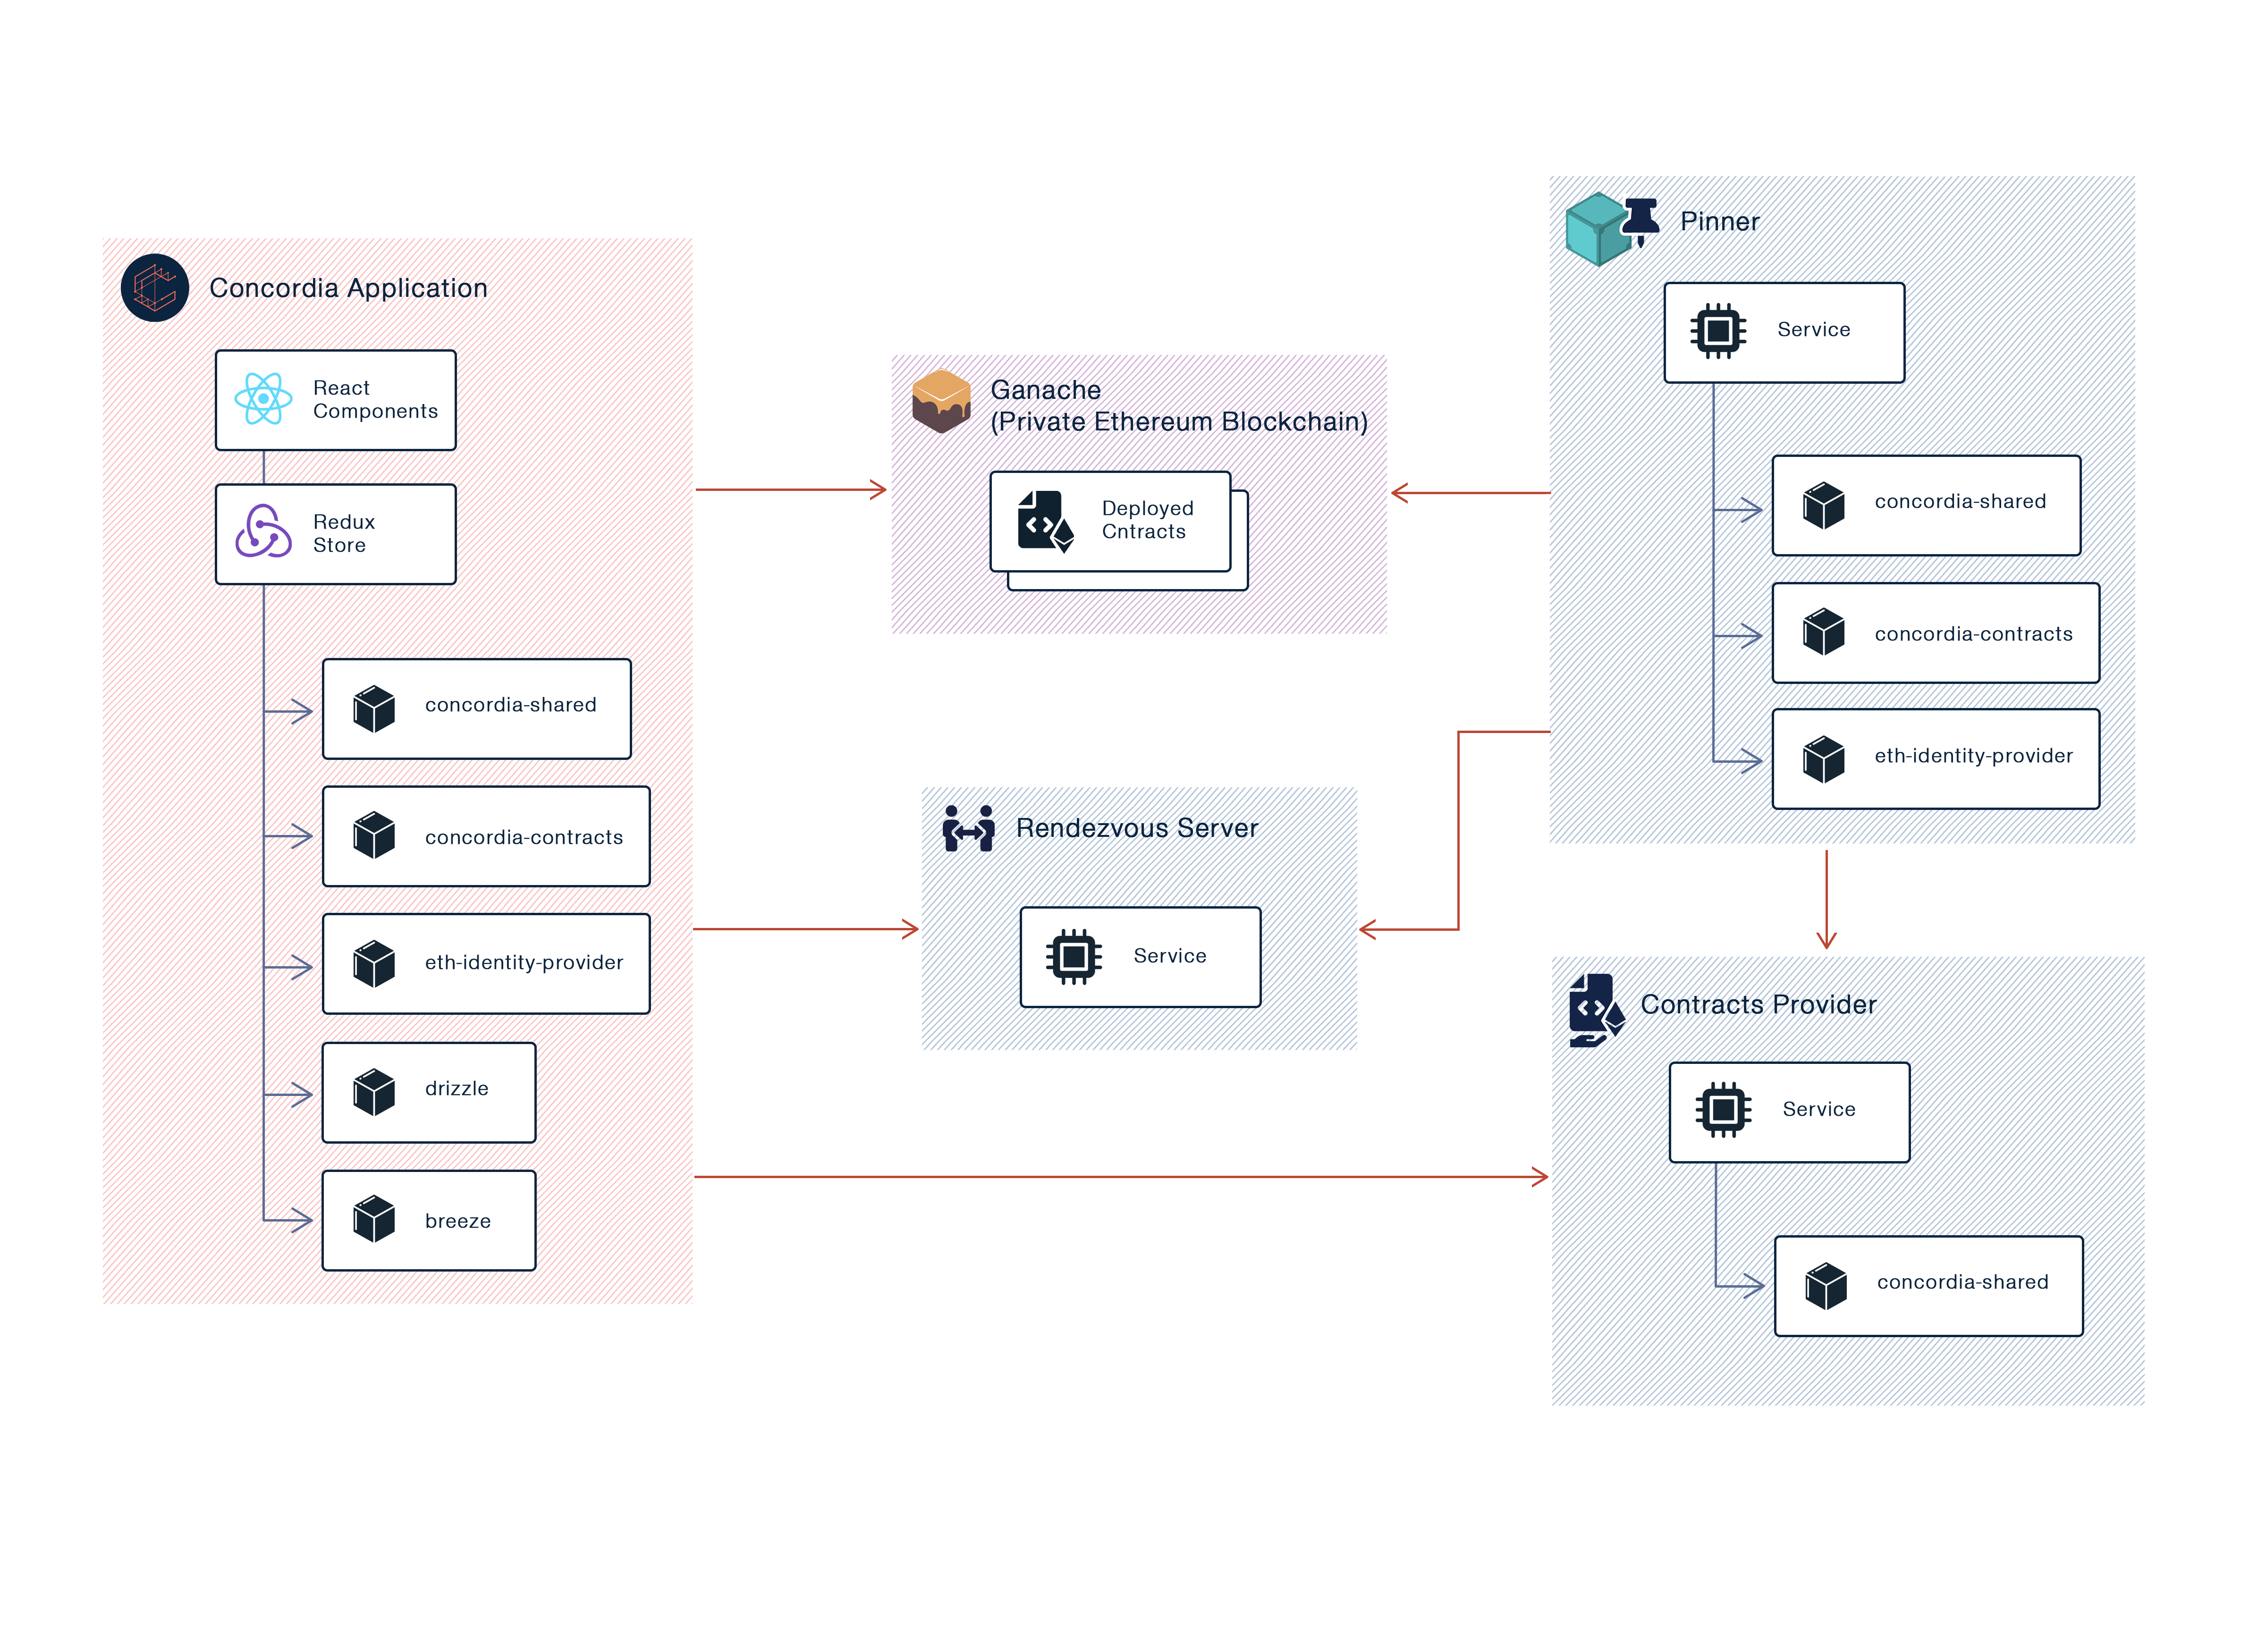
\includegraphics[width=\textwidth]{assets/figures/architecture-overview.png}
\end{frame}

\note{
	Εδώ θα δούμε τον τρόπο με τον οποίο χρησιμοποιήθηκαν οι τεχνολογίες που αναφέραμε προηγουμένως, την σχεδίαση της πλατφόρμας σε υψηλό επίπεδο καθώς και την αλληλεπίδραση των επιμέρους συστημάτων.

	Το βασικότερο μέρος της πλατφόρμας είναι η εφαρμογή (Concordia Application). Αυτό αποτελεί μία διαδικτυακή εφαρμογή με μορφή ιστοσελίδας. Εκθέτει τις γραφικές διεπαφές μέσω των οποίων αλληλεπιδρούν οι χρήστες με την πλατφόρμα. Στην εφαρμογή αυτή χρησιμοποιούνται αρθρώματα (διακριτά μέρη κώδικα) που διαχειρίζονται τις απαραίτητες διαδικασίες, όπως οι συναλλαγές με το blockchain και η αποθήκευση στο IPFS.

	Ο rendezvous server είναι ένα λογισμικό απαραίτητο για την χρήση του IPFS. Διατηρεί μία λίστα των διευθύνσεων των χρηστών που είναι ενεργοί στο σύστημα κάθε στιγμή, την οποία παρέχει σε νέους χρήστες που εισέρχονται σε αυτό. Έτσι, μέσω του server αυτού γίνεται η ανακάλυψη ομότιμων κόμβων (peer discovery).

	Η εφαρμογή pinner είναι ένα αυτόνομο λογισμικό το οποίο ανακαλύπτει νέα δεδομένα στο σύστημα, όπως χρήστες, μηνύματα ή polls, και αναλαμβάνει την επ' αόριστων αποθήκευσή τους ή το pinning. Πολλά instances της εφαρμογής αυτής μπορούν να εκτελούνται ταυτόχρονα σε διάφορα συστήματα ώστε να υπάρχει καλύτερη και αμεσότερη διαθεσιμότητα των δεδομένων.

	Τέλος, τα λογισμικά Ganache και Contracts Provider χρησιμοποιήθηκαν κατά την ανάπτυξη της πλατφόρμας αλλά δεν είναι απαραίτητα για την λειτουργία της. Το Ganache είναι ένα ιδιωτικό Ethereum blockchain, είναι δηλαδή ένα υποκατάστατο του πραγματικού Ethereum που χρησιμοποιείται κατά το development για την αποφυγή εξόδων. Το Contracts Provider είναι ένα σύστημα διανομής των απαραίτητων αρχείων για την εύρεση και χρήση των contracts από την εφαρμογή. Σε περιβάλλον πραγματικής χρήσης το Ganache θα αντικαθιστούνταν από το πραγματικό Ethereum blockchain και τα απαραίτητα αρχεία των contracts θα ήταν ενσωματωμένα στην εφαρμογή.
}

\section{Μέθοδοι και Χρονοδιάγραμμα Υλοποίησης}
\begin{frame}
	\frametitle{Μέθοδοι και Χρονοδιάγραμμα Υλοποίησης}

	\centering
	\includegraphics[width=.82\textwidth]{assets/figures/implementation-sprints.png}
\end{frame}

\note{
	Σε αυτό το μέρος της παρουσίασης θα αναλύσουμε τις μεθόδους που χρησιμοποιήθηκαν κατά την ανάπτυξη της εφαρμογής και τον χρονοπρογραμματισμό που έγινε.

	Τόσο η σχεδίαση όσο και η ανάπτυξη της εφαρμογής ακολούθησαν τις σύγχρονες μεθόδους Agile development.

	Το συνολικό έργο χωρίστηκε σε tasks. Τα tasks είναι αυτόνομα μέρη υλοποίησης που λύνουν ένα μικρό υπο-πρόβλημα της συνολικής σχεδίασης. Δημιουργήθηκαν οχτώ ομάδες, Sprints, οι οποίες αναφέρονται σε διακριτούς στόχους της πλατφόρμας και ομαδοποιούν τα tasks τα οποία συνεισφέρουν στον στόχο αυτό. Τα tasks κάθε ομάδας υλοποιήθηκαν παράλληλα. Ενώ οι ομάδες υλοποιήθηκαν διαδοχικά σε προδιαγεγραμμένο χρονικό ορίζοντα περάτωσης, καταλαμβάνοντας ένα μήνα ανάπτυξης η κάθε μία.

	Η πλειοψηφία των task αφορά στην υλοποίηση επιμέρους χαρακτηριστικών της πλατφόρμας όπως η εγγραφή ή η δημοσίευση μηνυμάτων.

	Έγινε επίσης δουλειά σε άλλα μέρη της ανάπτυξης όπως το DevOps. Για τις ανάγκες της υλοποίησης, έγινε χρήση του συστήματος CI-CD Jenkins. Το Jenkins είναι ένα αυτοματοποιημένο σύστημα ενσωμάτωσης, ελέγχου και ολοκλήρωσης λογισμικού. Με τη χρήση του CI-CD αυτοματοποιήθηκαν: το χτίσιμο (build) των εφαρμογών μας, ο έλεγχος (testing), η ενσωμάτωση που εδώ αφορά την δημοσίευση του πακεταρισμένου λογισμικού, καθώς και η εγκατάσταση (deployment).

	Λόγω χρονικών περιορισμών, αποφασίσαμε να μην προχωρήσουμε στην υλοποίηση του τελευταίου Sprint.
}

\section{Δυνατότητες Εφαρμογής}
\begin{frame}
	\frametitle{Δυνατότητες Εφαρμογής}
	\vspace{-\baselineskip}

	Δυνατότητες πλατφόρμας:
	\begin{itemize}
		\item Προσωπικά προφίλ (profiles)
		\item Δημιουργία θεμάτων (topics)
		\item Δημοσίευση μηνυμάτων (posts)
		\item Ψήφιση μηνυμάτων (upvote/downvote posts)
		\item Δημιουργία ψηφοφοριών (polls)
		\item Δημιουργία αυτόνομων κοινοτήτων (communities)
	\end{itemize}
\end{frame}

\note{
	Το αποτέλεσμα της προσπάθειας αυτής είναι μία αποκεντρωμένη πλατφόρμα επικοινωνίας που παρέχει όλες τις βασικές δυνατότητες αντίστοιχων κεντροποιημένων εφαρμογών.

	Οι χρήστες μπορούν να εγγραφούν δημιουργώντας προσωπικά προφίλ και έπειτα να δημοσιεύσουν θέματα και μηνύματα. Υλοποιήθηκαν επίσης οι δυνατότητες ψηφοφοριών σε μηνύματα αλλά και σε ξεχωριστά polls.

	Ένα χαρακτηριστικό που προδιαγράφηκε αλλά δεν υλοποιήθηκε λόγω των χρονικών περιορισμών που αναφέρθηκαν προηγουμένως είναι η δυνατότητα δημιουργίας ξεχωριστών κοινοτήτων μέσα στο σύστημα.
}

\section{Συμπεράσματα}
\begin{frame}
	\frametitle{Συμπεράσματα}
	\vspace{-\baselineskip}
	\begin{center}
		\includegraphics[width=.1\paperwidth]{assets/figures/concordia-logo}
	\end{center}
	\textbf{Concordia} - μία πλήρως αποκεντρωμένη αυτόνομη κοινωνική πλατφόρμα ...με ορισμένα εμπόδια:
	\begin{itemize}
		\item Πρώιμες τεχνολογίες
		\item Ethereum - τέλη συναλλαγών, συγκράτηση χρηστών, κλιμακοθετησιμότητα
		\item IPFS υβριδικό ως προς την ανακάλυψη κόμβων
	\end{itemize}
\end{frame}

\note{
	Καταλήγουμε έτσι στα συμπεράσματα της εργασίας.
	
	Όσον αφορά στον αρχικό στόχο, η πιλοτική μας εφαρμογή αποδεικνύει ότι ο σχεδιασμός μιας πλατφόρμας που να εκπληρώνει τους στόχους που τέθηκαν είναι εφικτός. Είναι δηλαδή εφικτή τόσο η κατοχύρωση της ελευθερίας του λόγου των χρηστών, όσο και η εξασφάλιση αυθεντικών δημοκρατικών διαδικασιών, μέσω των τεχνολογιών που επιλέχθηκαν.
	
	Ωστόσο, πρέπει να πούμε ότι υπάρχουν ορισμένα σημαντικά εμπόδια.
	
	Πρώτα απ' όλα και οι δύο τεχνολογίες είναι ακόμα πρώιμες. Αυτό σημαίνει ότι έχουμε ακόμα beta versions, διάφορες ελλείψεις και τεχνικά ζητήματα που δεν έχουν λυθεί.

	Όσον αφορά στο Ethereum, όπως έχουν τα πράγματα με τα τέλη των συναλλαγών και την \textit{ανάγκη χρήσης πρόσθετου λογισμικού} για τη σύνδεση με το blockchain, κάνουν ιδιαίτερα δύσκολο τόσο να υιοθετηθεί από τους χρήστες, όσο και αυτοί να παραμείνουν σε αυτό. Επίσης, πέρα από τη συγκράτηση των χρηστών, υπάρχει το θέμα της κλιμακοθετησιμότητας, με την έννοια ότι αυτή τη στιγμή επιτρέπονται σχετικά λίγες συναλλαγές ανά δευτερόλεπτο επί του Ethereum.
	
	Από την άλλη υπάρχει προς το παρόν το πρόβλημα ότι ως προς την ανακάλυψη κόμβων το IPFS λειτουργεί υβριδικά, απαιτείται δηλαδή μία σύνδεση με signalling nodes για την ανακάλυψη των κατάλληλων peer.
}
\section{Ανοιχτά Θέματα}
\begin{frame}
	\frametitle{Ανοιχτά Θέματα}
	\begin{itemize}
		\item Διαχείριση των τελών του Ethereum
		\item Διανομή των Ethereum token
		\item Εναλλακτικά συστήματα ψηφοφορίας
		\item Συστήματα απόδοσης εμπιστοσύνης
	\end{itemize}
\end{frame}

\note{
	Έτσι, φτάνουμε στα ανοιχτά θέματα.
	
	Το πρώτο και σημαντικότερο είναι η διαχείριση των τελών στις συναλλαγές του Ethereum. Αυτό που προτείνουμε και είναι γενικά η τάση που επικρατεί είναι η χρήση μετασυναλλαγών. Στην περίπτωσή μας αυτό θα σήμαινε π.χ. ότι η πληρωμή των τελών θα προωθείται από τον χρήστη στην κοινότητα που ανήκει.
	
	Ένα δεύτερο ζήτημα είναι η δημιουργία μηχανισμών για την ανώνυμη διανομή των token στους χρήστες. Αν και στην υλοποίησή μας αφήσαμε ανοιχτή τη διαδικασία διανομής των token στην εκάστοτε κοινότητα, θα πρέπει να τονίσουμε ότι σχετικά πρόσφατα άρχισαν να εμφανίζονται υλοποιήσεις στο Ethereum που μπορούν να ενσωματωθούν και που την απλοποιούν κατά πολύ, επιτρέποντας την ανώνυμη μετακίνηση token από διεύθυνση σε διεύθυνση.
	
	Επίσης, οι διαδικασίες των ψηφοφοριών μπορούν να επεκταθούν και να ορίζονται αυθαίρετα από την κάθε κοινότητα. Για παράδειγμα να υπάρχει επιλογή για ψηφοφορία με σειρά προτίμησης ή για έμμεση ψηφοφορία.
	
	Τέλος, μπορούν να χτιστούν συστήματα απόδοσης εμπιστοσύνης για τους χρήστες, τα οποία να λειτουργούν κυρίως συμπληρωματικά με τα θέματα των τελών και των ψηφοφοριών. Για παράδειγμα σε μία κοινότητα ένας χρήστης να απαλλάσσεται από τέλη εάν περάσει ένα όριο εμπιστοσύνης ή η ισχύς της ψήφου του να ορίζεται από αυτήν.
}

\section{Ερωτήσεις}
\begin{frame}
	\frametitle{Ερωτήσεις}
	\centering
	\Huge Ευχαριστούμε για την προσοχή σας!
\end{frame}


\end{document}
